\chapter{Entornos de Desarrollo}
\label{cap:EntornosDeDesarrollo}
\graphicspath{ {Imagenes/Figuras/} }


En este capítulo se van a enumerar una serie de librerías, herramientas, entornos y lenguajes
de programación que hemos utilizado y han facilitado la realización del proyecto.
También se procederá a explicar nuestro sistema de control de versiones y la base de datos empleada, además de las utilidades para prototipo de las interfaces.

\section{Frameworks y Librerías}
En esta sección se enumera la lista de entornos usados para el desarrollo de las dos aplicaciones, así como los \textit{frameworks} que nos han ayudado en la implementación del código.

\subsection{Visual Studio Code}

Visual Studio Code~\citep{VSCode} es un editor de código fuente desarrollado por Microsoft. Es un software libre y multiplataforma, que está disponible para Windows, GNU/Linux y macOS. VS Code tiene una buena integración con Git, cuenta con soporte para depuración de código, y dispone de un sin número de extensiones, que básicamente da la posibilidad de escribir y ejecutar código en cualquier lenguaje de programación.

\subsection{Android Studio}
Android Studio~\citep{AndroidStudio}, es el entorno de desarrollo integrado oficial del sistema operativo Android de Google, basado en el software IntelliJ IDEA de JetBrains y diseñado específicamente para el desarrollo de Android. Está disponible para su descarga en sistemas operativos basados en Windows, macOS y Linux. Además es el principal entorno de desarrollo para aplicaciones
móviles, con soporte para diversos lenguajes de programación como Java,
C++ y Kotlin.

\subsection{Maven}

Maven~\citep{Maven} es un \textit{Project Management Framework}, esto es, un \textit{framework} de gestión de proyectos de \textit{software}, que proporciona un modelo estándar de gestión y descripción de proyectos. Maven da soluciones a tareas que abarcan desde la compilación hasta la distribución, despliegue y documentación de los proyectos.

\subsection{Bootstrap}

Bootstrap~\citep{bootstrap} es un \textit{framework} CSS gratuito y de código abierto orientado al desarrollo web \textit{front-end} responsivo y \textit{mobile-first}. Contiene plantillas de diseño basadas en HTML, CSS y JavaScript para tipografía, formularios, botones, navegación y otros componentes de la interfaz.

\subsection{SweetAlert}

SweetAlert~\citep{sweetAlert} es una variante atractiva y muy personalizable para gestionar los \textit{pop-ups} emergentes en javascript.

\subsection{Docker}

Docker~\citep{docker} es un proyecto de código abierto que automatiza el despliegue de aplicaciones dentro de contenedores de software, proporcionando una capa adicional de abstracción y automatización de virtualización de aplicaciones en múltiples sistemas operativos.

\subsection{Fly.io}

Fly.io~\citep{fly.io} es una nueva nube pública, construida sobre servidores \textit{Bare-Metal} que se gestiona en centros de datos de todo el mundo, diseñada para facilitar el despliegue de aplicaciones distribuidas y en tiempo real cerca de sus usuarios, estén donde estén.

\section{Lenguajes de Programación}
Durante la realización del proyecto se han utilizado los lenguajes de programación presentados a continuación.

\subsection{HTML}

HTML~\citep{html} es el lenguaje de marcado estándar para documentos diseñados para visualizarse en un navegador web. Suele estar asistido por tecnologías como las hojas de estilo en cascada \textit{(Cascading Style Sheets)} y lenguajes de script como JavaScript.

\subsection{CSS}

CSS~\citep{css} es un lenguaje que permite el desarrollo del estilo de una página web cuando es utilizado sobre otro lenguaje de marcado, como en este caso HTML. Aunque la mayor parte del aspecto visual de la aplicación está realizado a través de Bootstrap se han incluido algunas hojas de estilo para añadir detalles que este \textit{framework} no contempla.

\subsection{Javascript}

JavaScript~\citep{javascript} es un lenguaje de programación que se utiliza para hacer páginas web interactivas. Desde actualizar fuentes de redes sociales a mostrar animaciones y mapas interactivos, las funciones de JavaScript pueden mejorar la experiencia del usuario de un sitio web.

\subsection{Java}

Java~\citep{java} es un lenguaje de programación ampliamente utilizado para codificar aplicaciones web. Ha sido una opción popular entre los desarrolladores durante más de dos décadas, con millones de aplicaciones Java en uso en la actualidad.

\subsection{Kotlin}

Kotlin~\citep{kotlin} es un lenguaje de programación de código abierto creado por JetBrains que se ha popularizado gracias a que se puede utilizar para programar aplicaciones Android.

\section{Bases de Datos}

Como gestor de base de datos decidimos usar \textit{Firebase} debido a su comodidad para integrarse en aplicaciones móviles realizadas con Android Studio.


Cloud Firestore~\citep{firestore} es una base de datos NoSQL orientada a documentos. A diferencia de una base de datos SQL, no hay tablas. En su lugar, se almacenan los datos en documentos, que se organizan en colecciones. Cada documento contiene un conjunto de pares clave-valor. En la Figura~\ref{fig:erd} podemos observar el diagrama entidad-relación

\begin{figure}[h]
\centering
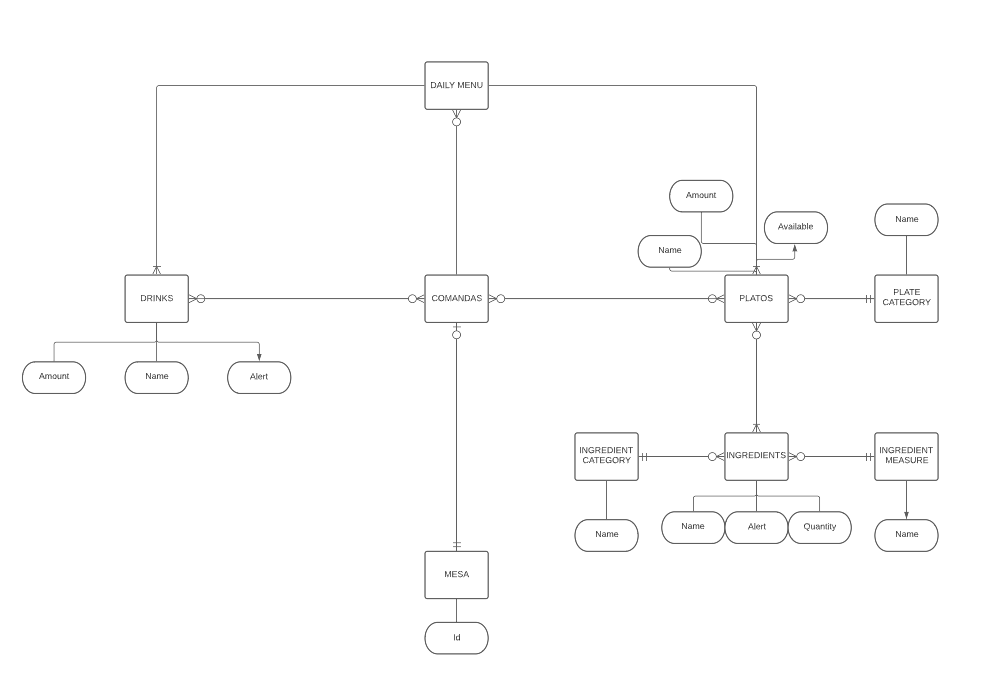
\includegraphics[width=16cm, height=13cm]{Imagenes/Figuras/ERD.png}
\caption{Diagrama entidad relación}\label{fig:erd}
\end{figure} 


\section{Control de Versiones}

GitHub~\citep{github} ofrece un servicio, tanto gratuito como de pago, para el control de versiones de proyectos usando la tecnología Git, registrando cada cambio subido al servidor gracias a su almacenamiento en la nube, y permitiendo volver a versiones anteriores o comparar los cambios realizados entre las mismas.
Decidimos usar esta plataforma dada nuestra experiencia con ella y que nos viene muy bien para trabajar paralelamente los proyectos.
Para ello creamos dos repositorios, uno para el desarrollo de la aplicación móvil, Figura~\ref{fig:githubapp}, y otro para el de la web, Figura~\ref{fig:githubweb}.

\begin{itemize}

\item Aplicación movil: 
\url{https://github.com/jesusmoraleda/TakeOrder.git}. 

\begin{figure}[h]
\centering
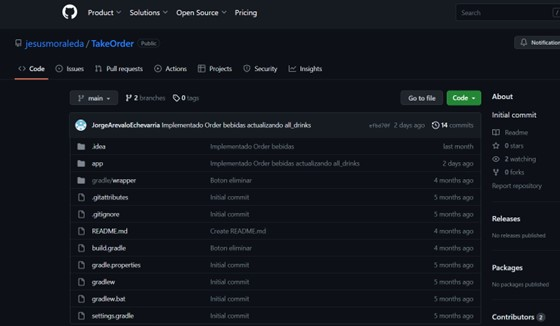
\includegraphics[width=13cm, height=8cm]{Imagenes/Figuras/GitHubAppMovil.jpg}
\caption{Repositorio del código de la aplicación}\label{fig:githubapp}
\end{figure} 



\item Aplicación web: 
\url{https://github.com/jesusmoraleda/TakeOrderAdmin.git}. 

\end{itemize}


\begin{figure}[h]
\centering
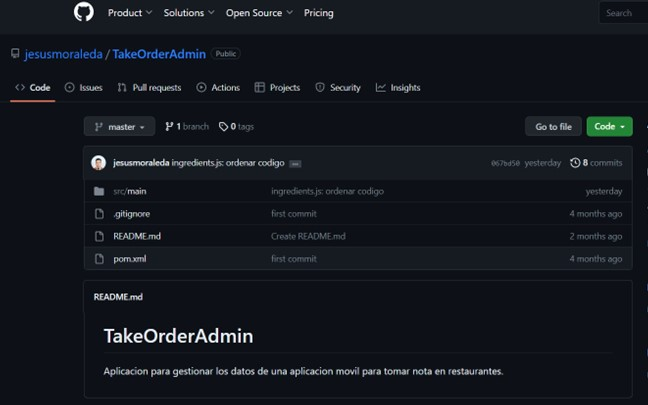
\includegraphics[width=13cm, height=8cm]{Imagenes/Figuras/GitHubAppWeb.jpg}
\caption{Repositorio del código web}\label{fig:githubweb}
\end{figure} 


\section{Maquetación y Prototipos}
Comenzamos desarrollando unos \textit{mockups} para que nos ayudaran a tener una idea general del aspecto que queríamos para la app móvil, como las que aparecen en las Figuras~\ref{fig:mockup1} y~\ref{fig:mockup2}, y para aplicación web como se puede visualizar en la Figura~\ref{fig:mockupWeb}, con el objetivo de resultar amistosa para el usuario.


\begin{figure}[h]
 \centering
  \subfloat[Mockup 1]{\label{fig:mockup1}
   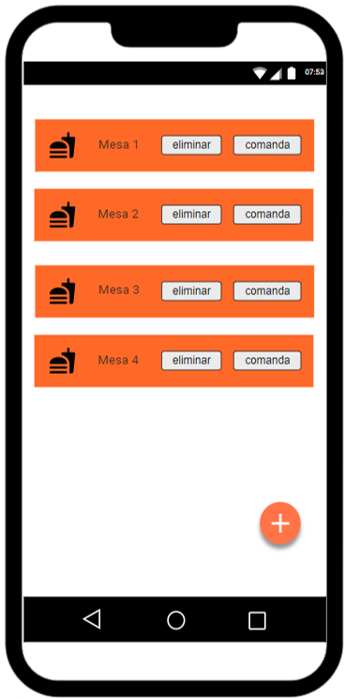
\includegraphics[width=4cm, height=8cm]{Imagenes/Figuras/mockup1.png}}
    \hfill
  \subfloat[Mockup 2]{\label{fig:mockup2}
    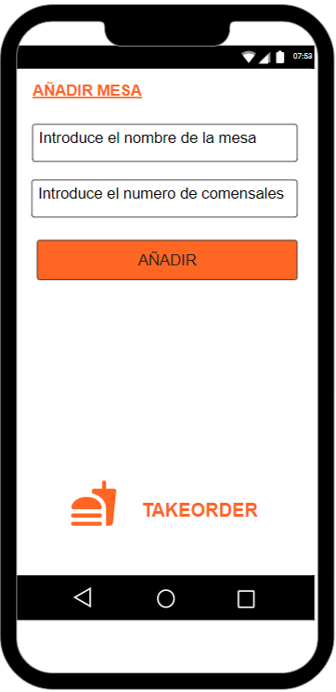
\includegraphics[width=4cm, height=8cm]{Imagenes/Figuras/mockup2.png}}
 \caption{Mockup aplicación Móvil}
\label{fig:mockupAppMovil}
\end{figure}

\begin{figure}[h]
 \centering
\scalebox{0.75}{ 
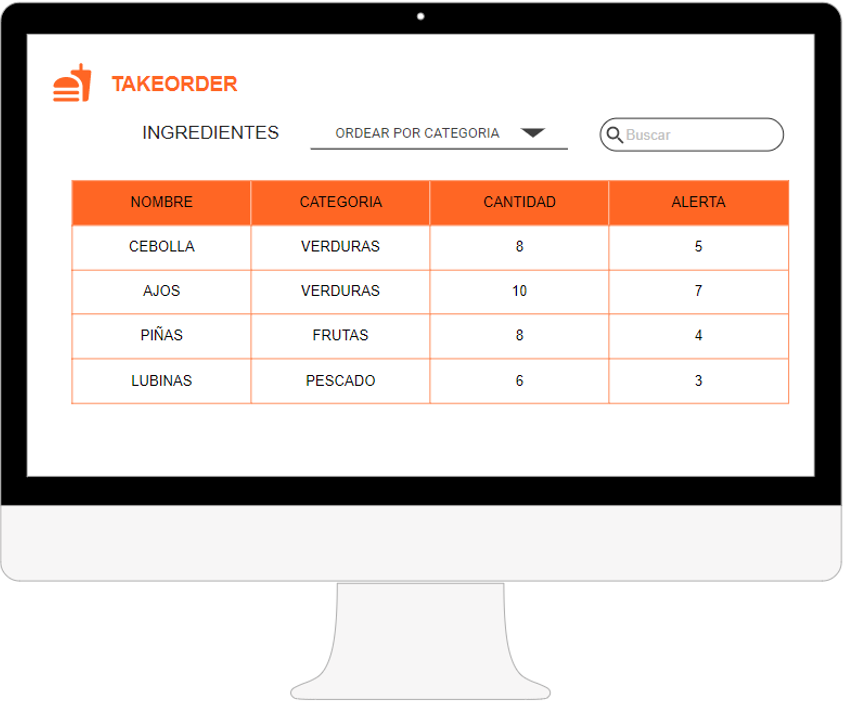
\includegraphics[width=11cm, height=9cm]{Imagenes/Figuras/mockupWeb.png}}
\caption{Mockup aplicación web}\label{fig:mockupWeb}
\end{figure} 


